\documentclass[11pt,letter]{article}\usepackage[]{graphicx}\usepackage[]{color}
%% maxwidth is the original width if it is less than linewidth
%% otherwise use linewidth (to make sure the graphics do not exceed the margin)
\makeatletter
\def\maxwidth{ %
  \ifdim\Gin@nat@width>\linewidth
    \linewidth
  \else
    \Gin@nat@width
  \fi
}
\makeatother

\definecolor{fgcolor}{rgb}{0.345, 0.345, 0.345}
\newcommand{\hlnum}[1]{\textcolor[rgb]{0.686,0.059,0.569}{#1}}%
\newcommand{\hlstr}[1]{\textcolor[rgb]{0.192,0.494,0.8}{#1}}%
\newcommand{\hlcom}[1]{\textcolor[rgb]{0.678,0.584,0.686}{\textit{#1}}}%
\newcommand{\hlopt}[1]{\textcolor[rgb]{0,0,0}{#1}}%
\newcommand{\hlstd}[1]{\textcolor[rgb]{0.345,0.345,0.345}{#1}}%
\newcommand{\hlkwa}[1]{\textcolor[rgb]{0.161,0.373,0.58}{\textbf{#1}}}%
\newcommand{\hlkwb}[1]{\textcolor[rgb]{0.69,0.353,0.396}{#1}}%
\newcommand{\hlkwc}[1]{\textcolor[rgb]{0.333,0.667,0.333}{#1}}%
\newcommand{\hlkwd}[1]{\textcolor[rgb]{0.737,0.353,0.396}{\textbf{#1}}}%
\let\hlipl\hlkwb

\usepackage{framed}
\makeatletter
\newenvironment{kframe}{%
 \def\at@end@of@kframe{}%
 \ifinner\ifhmode%
  \def\at@end@of@kframe{\end{minipage}}%
  \begin{minipage}{\columnwidth}%
 \fi\fi%
 \def\FrameCommand##1{\hskip\@totalleftmargin \hskip-\fboxsep
 \colorbox{shadecolor}{##1}\hskip-\fboxsep
     % There is no \\@totalrightmargin, so:
     \hskip-\linewidth \hskip-\@totalleftmargin \hskip\columnwidth}%
 \MakeFramed {\advance\hsize-\width
   \@totalleftmargin\z@ \linewidth\hsize
   \@setminipage}}%
 {\par\unskip\endMakeFramed%
 \at@end@of@kframe}
\makeatother

\definecolor{shadecolor}{rgb}{.97, .97, .97}
\definecolor{messagecolor}{rgb}{0, 0, 0}
\definecolor{warningcolor}{rgb}{1, 0, 1}
\definecolor{errorcolor}{rgb}{1, 0, 0}
\newenvironment{knitrout}{}{} % an empty environment to be redefined in TeX

\usepackage{alltt}    
%\usepackage[latin1]{inputenc}
\usepackage[parfill]{parskip} % Activate to begin paragraphs with an empty line rather than an indent
\usepackage{amsmath,amsthm,amssymb,bbm} %math stuff
\usepackage{ctable}
\usepackage{placeins} % FloatBarrier
\usepackage{fancyhdr}
\usepackage{lastpage}
\usepackage{float}    % for fig.pos='H'
\usepackage{rotfloat} % for sidewaysfigure
%\usepackage{subfig}   % for subfigure
\usepackage{subcaption}  % an alternative package for sub figures
\newcommand{\subfloat}[2][need a sub-caption]{\subcaptionbox{#1}{#2}}
\usepackage{comment}
\usepackage[round]{natbib}   % omit 'round' option if you prefer square brackets
\bibliographystyle{plainnat}
\usepackage{setspace} %Spacing
\usepackage{graphicx,graphics}
\usepackage{booktabs,tabularx}
\usepackage{enumerate}
\usepackage{makecell}
\usepackage{xfrac}
\usepackage{color, colortbl, xcolor}
\usepackage{booktabs,dcolumn} % for use with texreg in R
\usepackage[pagebackref=true,bookmarks]{hyperref}
\hypersetup{
    unicode=false,          
    pdftoolbar=true,        
    pdfmenubar=true,        
    pdffitwindow=false,     % window fit to page when opened
    pdfstartview={FitH},    % fits the width of the page to the window
    pdftitle={004-Figures},    % title
    pdfauthor={SRB},     % author
    pdfsubject={Subject},   % subject of the document
    pdfcreator={SRB},   % creator of the document
    pdfproducer={SRB}, % producer of the document
    pdfkeywords={}, % list of keywords
    pdfnewwindow=true,      % links in new window
    colorlinks=true,       % false: boxed links; true: colored links
    linkcolor=red,          % color of internal links (change box color with linkbordercolor)
    citecolor=blue,        % color of links to bibliography
    filecolor=black,      % color of file links
    urlcolor=cyan           % color of external links
}

% my commands
\newcommand{\tm}[1]{\textrm{#1}}
\newtheorem{rexample}{R Example}[section]


% fancy header commands
\renewcommand{\headrulewidth}{0.0pt}
\renewcommand{\footrulewidth}{0.0pt}
\setlength{\textheight}{9.00in}
\setlength{\textwidth}{7.00in}
\setlength{\topmargin}{-0.5in}
\setlength{\evensidemargin}{-0.25in}
\setlength{\oddsidemargin}{-0.25in}
\renewcommand{\baselinestretch}{1.2}
\makeatletter
\makeatother
\lfoot{} \cfoot{ } \rfoot{{\small{\em Page \thepage \ of \pageref{LastPage}}}}
\IfFileExists{upquote.sty}{\usepackage{upquote}}{}
\begin{document}
\pagestyle{fancy}

\title{002-Minimum Working Example}
\author{}
\maketitle






\begin{abstract}
We familiarize ourselves with the basics of \texttt{knitr}~\citep{k1,k2,k3}; including plots, tables and code. 
\end{abstract}

\section{Figures}

The first example is given by~\ref{fig1}

\begin{knitrout}
\definecolor{shadecolor}{rgb}{0.969, 0.969, 0.969}\color{fgcolor}\begin{kframe}
\begin{rexample}\label{fig1}\hfill{}\begin{alltt}
\hlkwd{par}\hlstd{(}\hlkwc{mar} \hlstd{=} \hlkwd{c}\hlstd{(}\hlnum{4}\hlstd{,} \hlnum{4}\hlstd{,} \hlnum{0.1}\hlstd{,} \hlnum{0.1}\hlstd{))}
\hlstd{x} \hlkwb{=} \hlkwd{rnorm}\hlstd{(}\hlnum{100}\hlstd{)}
\hlkwd{hist}\hlstd{(x,} \hlkwc{main} \hlstd{=} \hlstr{""}\hlstd{,} \hlkwc{col} \hlstd{=} \hlstr{"lightblue"}\hlstd{,} \hlkwc{border} \hlstd{=} \hlstr{"white"}\hlstd{)}
\hlkwd{rug}\hlstd{(x)}
\end{alltt}
\end{rexample}\end{kframe}
\end{knitrout}


\begin{knitrout}
\definecolor{shadecolor}{rgb}{0.969, 0.969, 0.969}\color{fgcolor}\begin{kframe}
\begin{rexample}\label{fig2}\hfill{}\begin{alltt}
\hlkwd{plot}\hlstd{(cars,} \hlkwc{pch} \hlstd{=} \hlnum{20}\hlstd{,} \hlkwc{col} \hlstd{=} \hlstr{"darkgray"}\hlstd{)}
\hlstd{fit} \hlkwb{<-} \hlkwd{lm}\hlstd{(dist} \hlopt{~} \hlstd{speed,} \hlkwc{data} \hlstd{= cars)}
\hlkwd{abline}\hlstd{(fit,} \hlkwc{lwd} \hlstd{=} \hlnum{2}\hlstd{)}
\end{alltt}
\end{rexample}\end{kframe}
\end{knitrout}

\begin{knitrout}
\definecolor{shadecolor}{rgb}{0.969, 0.969, 0.969}\color{fgcolor}\begin{kframe}
\begin{rexample}\label{fig3}\hfill{}\begin{alltt}
\hlkwd{par}\hlstd{(}\hlkwc{mfrow} \hlstd{=} \hlkwd{c}\hlstd{(}\hlnum{2}\hlstd{,} \hlnum{2}\hlstd{))}
\hlkwd{plot}\hlstd{(fit)}
\end{alltt}
\end{rexample}\end{kframe}
\end{knitrout}


\section{Tables}

\begin{knitrout}
\definecolor{shadecolor}{rgb}{0.969, 0.969, 0.969}\color{fgcolor}\begin{kframe}
\begin{rexample}\label{table-1}\hfill{}\begin{alltt}
\hlstd{fit} \hlkwb{<-} \hlkwd{lm}\hlstd{(dist} \hlopt{~} \hlstd{speed,} \hlkwc{data} \hlstd{= cars)}
\hlkwd{summary}\hlstd{(fit)}
\hlstd{xtable}\hlopt{::}\hlkwd{xtable}\hlstd{(fit,} \hlkwc{digits} \hlstd{=} \hlnum{2}\hlstd{)}
\end{alltt}
\end{rexample}\end{kframe}
\end{knitrout}


\begin{knitrout}
\definecolor{shadecolor}{rgb}{0.969, 0.969, 0.969}\color{fgcolor}\begin{kframe}
\begin{rexample}\label{table-2}\hfill{}\begin{alltt}
\hlcom{# %>% is the pipe operator from the magrittr library}
\hlstd{cars} \hlopt \hlkwd{summary}\hlstd{()} \hlopt \hlstd{xtable}
\end{alltt}
\end{rexample}\end{kframe}
\end{knitrout}

\begin{knitrout}
\definecolor{shadecolor}{rgb}{0.969, 0.969, 0.969}\color{fgcolor}\begin{kframe}
\begin{alltt}
\hlkwd{plot}\hlstd{(mtcars)}
\end{alltt}
\end{kframe}

{\centering 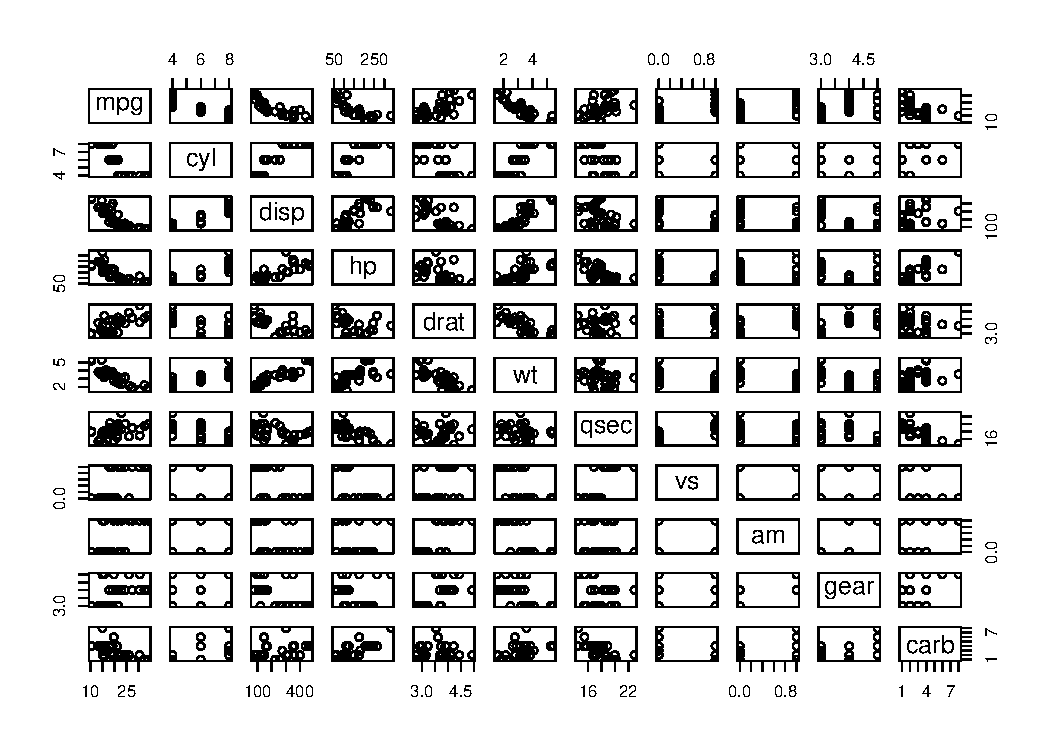
\includegraphics[width=\maxwidth]{figure/figure-1-1} 

}



\end{knitrout}







\newpage
\nocite{xtable,mag}
\bibliography{002-bibliography}


\newpage
\appendix

\section{R Code}
\begin{knitrout}
\definecolor{shadecolor}{rgb}{0.969, 0.969, 0.969}\color{fgcolor}\begin{kframe}
\begin{alltt}
\hlkwd{par}\hlstd{(}\hlkwc{mar} \hlstd{=} \hlkwd{c}\hlstd{(}\hlnum{4}\hlstd{,} \hlnum{4}\hlstd{,} \hlnum{0.1}\hlstd{,} \hlnum{0.1}\hlstd{))}
\hlstd{x} \hlkwb{=} \hlkwd{rnorm}\hlstd{(}\hlnum{100}\hlstd{)}
\hlkwd{hist}\hlstd{(x,} \hlkwc{main} \hlstd{=} \hlstr{""}\hlstd{,} \hlkwc{col} \hlstd{=} \hlstr{"lightblue"}\hlstd{,} \hlkwc{border} \hlstd{=} \hlstr{"white"}\hlstd{)}
\hlkwd{rug}\hlstd{(x)}
\hlkwd{plot}\hlstd{(cars,} \hlkwc{pch} \hlstd{=} \hlnum{20}\hlstd{,} \hlkwc{col} \hlstd{=} \hlstr{"darkgray"}\hlstd{)}
\hlstd{fit} \hlkwb{<-} \hlkwd{lm}\hlstd{(dist} \hlopt{~} \hlstd{speed,} \hlkwc{data} \hlstd{= cars)}
\hlkwd{abline}\hlstd{(fit,} \hlkwc{lwd} \hlstd{=} \hlnum{2}\hlstd{)}
\hlkwd{par}\hlstd{(}\hlkwc{mfrow} \hlstd{=} \hlkwd{c}\hlstd{(}\hlnum{2}\hlstd{,} \hlnum{2}\hlstd{))}
\hlkwd{plot}\hlstd{(fit)}
\hlstd{fit} \hlkwb{<-} \hlkwd{lm}\hlstd{(dist} \hlopt{~} \hlstd{speed,} \hlkwc{data} \hlstd{= cars)}
\hlkwd{summary}\hlstd{(fit)}
\hlstd{xtable}\hlopt{::}\hlkwd{xtable}\hlstd{(fit,} \hlkwc{digits} \hlstd{=} \hlnum{2}\hlstd{)}
\hlcom{# %>% is the pipe operator from the magrittr library}
\hlstd{cars} \hlopt \hlkwd{summary}\hlstd{()} \hlopt \hlstd{xtable}
\hlkwd{plot}\hlstd{(mtcars)}
\hlkwd{print}\hlstd{(}\hlkwd{sessionInfo}\hlstd{(),} \hlkwc{locale} \hlstd{=} \hlnum{FALSE}\hlstd{)}
\hlcom{######################################################### R Source code file for required packages for}
\hlcom{######################################################### 002-minimum-working-example.Rmd/Rnw Hosted on github repo}
\hlcom{######################################################### 'sahirbhatnagar/raqc' Author: Sahir Bhatnagar Created: May}
\hlcom{######################################################### 31, 2018 Updated: Notes: we use pacman to install packages.}
\hlcom{######################################################### p_load will check if the package is installed, install and}
\hlcom{######################################################### load it}
\hlkwa{if} \hlstd{(}\hlopt{!}\hlkwd{require}\hlstd{(}\hlstr{"pacman"}\hlstd{))} \hlkwd{install.packages}\hlstd{(}\hlstr{"pacman"}\hlstd{)}

\hlstd{pacman}\hlopt{::}\hlkwd{p_load}\hlstd{(knitr, here, xtable, dplyr, data.table)}
\hlkwd{head}\hlstd{(mtcars)}
\end{alltt}
\end{kframe}
\end{knitrout}

\newpage

\section{Session Information}
\begin{knitrout}
\definecolor{shadecolor}{rgb}{0.969, 0.969, 0.969}\color{fgcolor}\begin{kframe}
\begin{alltt}
\hlkwd{print}\hlstd{(}\hlkwd{sessionInfo}\hlstd{(),} \hlkwc{locale} \hlstd{=} \hlnum{FALSE}\hlstd{)}
\end{alltt}
\begin{verbatim}
## R version 3.6.0 (2019-04-26)
## Platform: x86_64-pc-linux-gnu (64-bit)
## Running under: Pop!_OS 18.10
## 
## Matrix products: default
## BLAS:   /usr/lib/x86_64-linux-gnu/blas/libblas.so.3.8.0
## LAPACK: /usr/lib/x86_64-linux-gnu/lapack/liblapack.so.3.8.0
## 
## attached base packages:
## [1] stats     graphics  grDevices utils     datasets 
## [6] methods   base     
## 
## other attached packages:
## [1] data.table_1.12.0 dplyr_0.8.0.1     xtable_1.8-4     
## [4] here_0.1          pacman_0.5.0      knitr_1.22       
## 
## loaded via a namespace (and not attached):
##  [1] Rcpp_1.0.1       crayon_1.3.4     rprojroot_1.3-2 
##  [4] assertthat_0.2.1 R6_2.4.0         backports_1.1.3 
##  [7] formatR_1.6      magrittr_1.5     evaluate_0.13   
## [10] highr_0.8        pillar_1.3.1     rlang_0.3.4     
## [13] stringi_1.4.3    tools_3.6.0      stringr_1.4.0   
## [16] glue_1.3.1       purrr_0.3.2      xfun_0.6        
## [19] compiler_3.6.0   pkgconfig_2.0.2  tidyselect_0.2.5
## [22] tibble_2.1.1
\end{verbatim}
\end{kframe}
\end{knitrout}


\end{document}
